De los resultados obtenidos a lo largo de este informe, vemos que los modelos más prometedores parecen ser aquellos basados en los algoritmos de \textit{linear discriminant analysis} y \textit{support vector machines}. En la búsqueda aleatoria ambos obtuvieron buenos puntajes. El anterior obtuvo un \textit{aucroc} promedio de $0.8649$ y el posterior de $0.8960$.

A pesar de la ventaja aparente del segundo, en el diagnóstico de sesgo y varianza continuamos por observar el comportamiento de ambos y notamos que el modelo basado en el algoritmo de \textit{support vector machines} parece tener un sesgo mayor y una tendencia a sobreajustarse a los datos, incluso al contar con una cantidad de datos grande de entrenamiento.

Luego, consideramos que el mejor modelo ---tanto en el sentido del \textit{aucroc} promedio, como en el sentido de la confianza que nuestra experimentación nos permite depositar en esta métrica--- es aquel obtenido por el algoritmo de \textit{linear discriminant analysis} con los hiperparámetros encontrados.  

Procedimos, finalmente, a entrenar un único modelo a través de este algoritmo con todos los datos de entrenamiento. Las Figuras \ref{metricas_final} y \ref{curvas_final} muestran su performance en evaluación. Estos valores conforman nuestra estimación empírica del poder de generalización del modelo.

Importa notar que hubo una pérdida de $6\%$ con respecto al mejor resultado obtenido durante validación. Sin embargo, esto es esperable, dado que la validación cruzada fue parte del proceso de entrenamiento y, por ende, da una mirada optimista de la performance real del modelo.

\vspace{0.5em}
\begin{figure}[!htbp]
    \begin{center}
        \begin{tabular}{ |c|c| } 
         \hline
        Métrica         & Valor \\
        \hline
        accuracy (test) &  0.8235 \\
        auprc (test)    &  0.7647 \\
        aucroc (test)   &  0.8321 \\
        \hline
        \end{tabular}
    \end{center}
    \caption{\textit{Accuracy}, \textit{aucroc} y \textit{auprc} obtenidos para el modelo final, evaluado sobre $D_{test}$} \label{metricas_final}
\end{figure}

\begin{figure}[!htbp]
    \centering 
    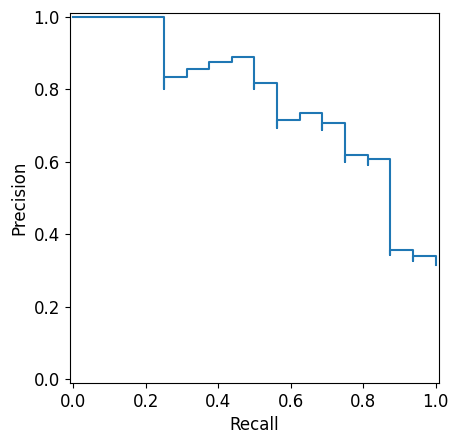
\includegraphics[width=0.45\textwidth]{/files/src/.media/finalAuprc.png}
    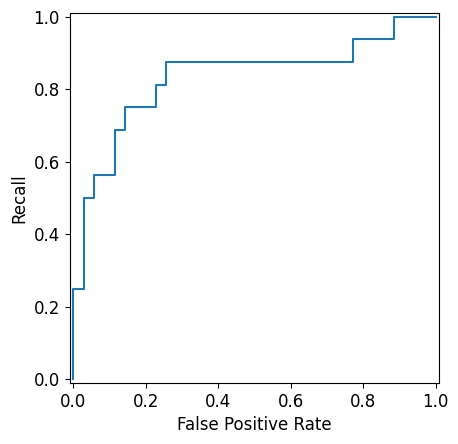
\includegraphics[width=0.45\textwidth]{/files/src/.media/finalAucroc.png}
    \caption{Curvas \textit{precision-recall}, izquierda, y \textit{receiving operator characteristic}, derecha, para el modelo final.}
    \label{curvas_final}
\end{figure}
